\section{Analysis}

Once the code has been completed and the functionality has been verified (See section xxx for verification) we have automated the process to run the application for every possible input size 1<=size<=128 and collect all the timing information to conduct performance analysis and get more insight into the application's behavior under different input sizes.



\begin{figure}[h!]
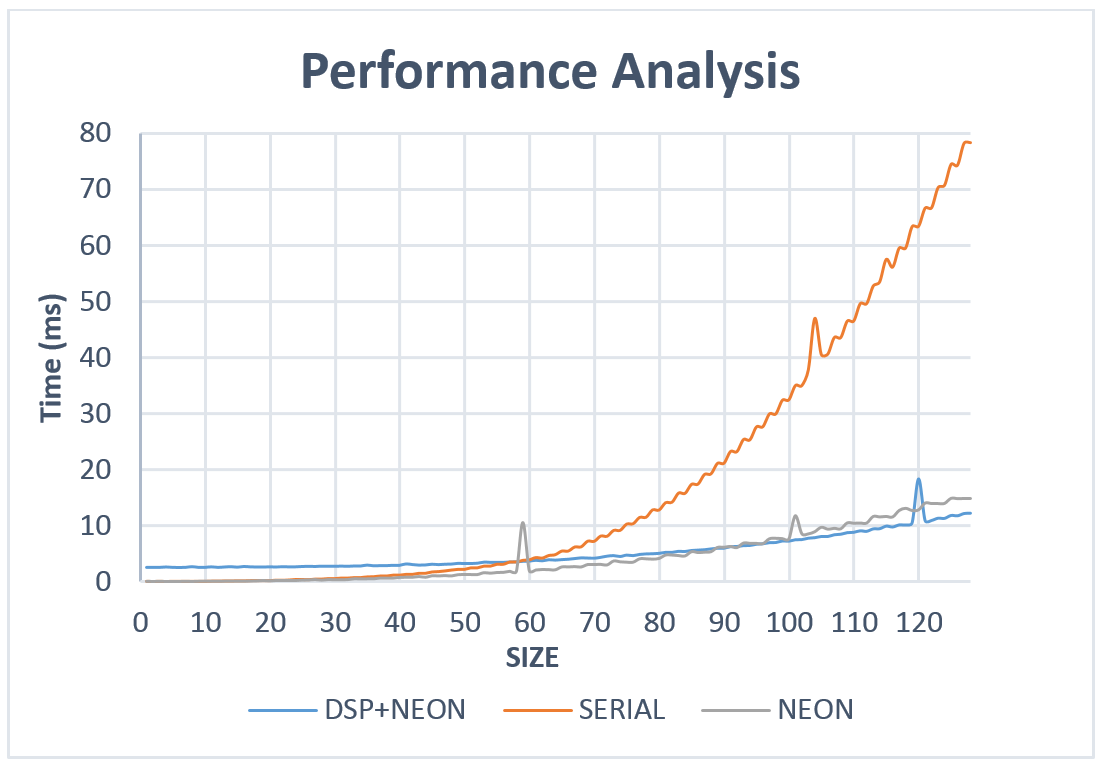
\includegraphics[width=\textwidth]{analysis/perf_plot}
\caption{Performance Analysis plot: Execution times as a function of input size for different configurations}
\label{fig:perf_plot}
\end{figure}


\begin{figure}[h!]
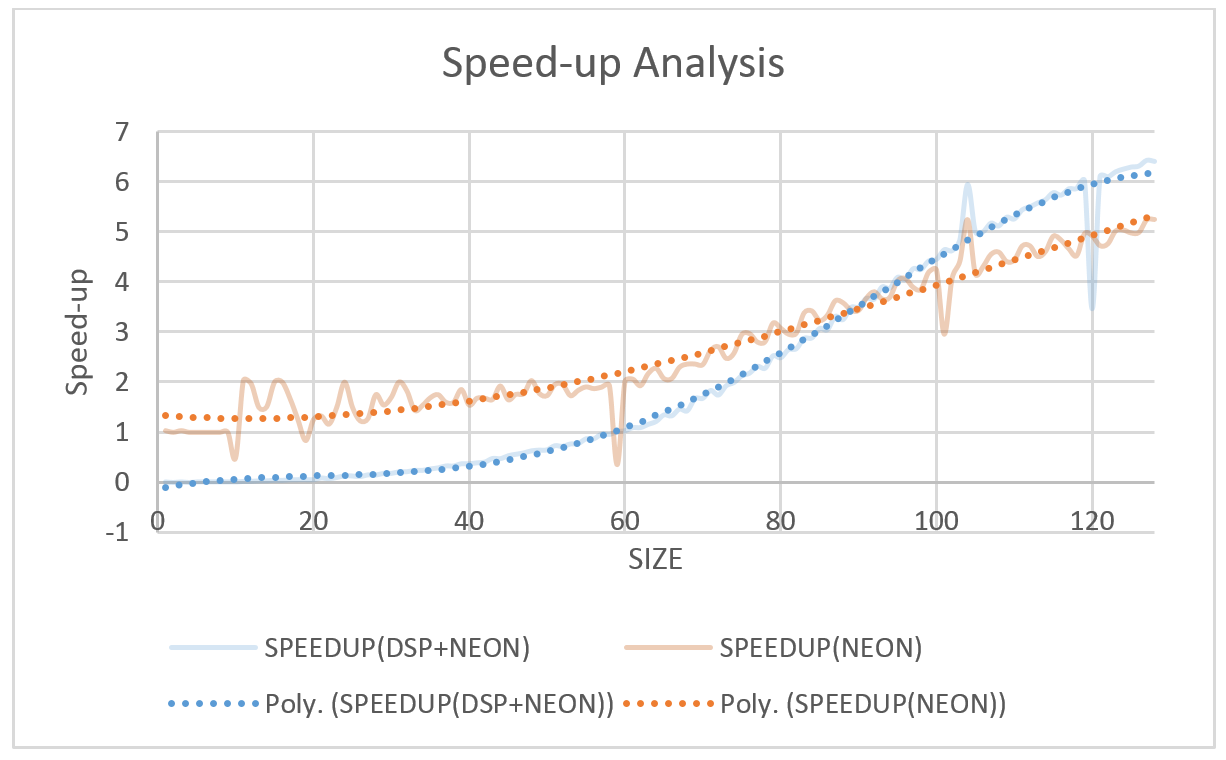
\includegraphics[width=\textwidth]{analysis/speedup_plot}
\caption{Speed-up plot: Achievable speed-up as a function of input size for different configurations}
\label{fig:speedup_plot}
\end{figure}

